A tensor 
\begin{center}
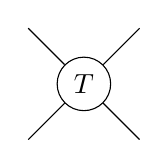
\begin{tikzpicture}
	\node[draw, circle] (T) at (0,0) {$T$};
	\foreach \x in {45,135,225,315}{
		\draw (T.\x) -- (\x:1cm);
		}
\end{tikzpicture}
\end{center}
is called \emph{perfect} if \underline{any} balanced bipartition of its legs yields a unitary transformation, up to a nonzero scalar. This notion was introduced in \cite{Pastawski2015Holographic}, but for the first part of that paper it is trivially true that a weaker requirement still gives rise to such things as the Ryu-Takayanagi formula for a connected bipartite boundary region. This weaker form shall be called a \emph{planarly perfect tensor}, implying that we only take balanced planar bipartitions into account --- that is, partitions of the indices into two sets of the same size so that all indices have at least one `neighbor' in their respective set. 

In this paper we argue that a construction of larger planarly perfect tensors from smaller ones exists. A complete proof of this particular construction can be found in the master's thesis of the first author, \cite{berger2017PerfectPlanarTangles}, where planarly perfect tensors were formalized in the more general setting of Jones' \emph{planar algebras} \cite{jones1999planar1}.

We will show this using a simple example that exhibits the basic idea behind the construction. More concretely, it is easy to see that
\begin{center}
\begin{tikzpicture}
			\node[draw] (T1) at (0.4,1) {${T}$};
			\node[draw] (T2) at (0,0) {${T}$};
			\node[draw] (T3) at (0.4,-1) {${T}$};
			
		
			\draw ($(T2.north) - (0.2,0)$) -- ($(T2.north |- T1.north) + (-0.2, 0.5)$);
			\draw ($(T2.south) - (0.2,0)$) -- ($(T2.south |- T3.south) + (-0.2, -0.5)$);
			\foreach \x in {0.2,-0.2}{
				\draw ($(T1.north) + (\x,0)$) -- ++ (0,0.5);
				\draw ($(T3.south) + (\x,0)$) -- ++ (0,-0.5);
				} 
			\draw ($(T2.north) + (0.2,0)$) -- ($(T1.south) + (-0.2,0)$);
			\draw ($(T2.south) + (0.2,0)$) -- ($(T3.north) + (-0.2,0)$);
			\draw ($(T3.north) + (0.2,0)$) -- ($(T1.south) + (0.2,0)$);
\end{tikzpicture}
\end{center}
also has this \emph{planar multi-unitarity} property, given that $T$ itself satisfies it. We will show the calculations in detail.

\bigno
Before doing so, we want to quickly exhibit where the intuition comes from. In the Temperley-Lieb algebra on $2$ strands with loop parameter $q$, $TL_2(q)$, the \emph{perfect} elements give rise to a representation of the braid group. We can thus make sense of diagrams such as
\begin{center}
\begin{tikzpicture}[scale=0.7]
	\braid[number of strands = 3] s_2 s_1 s_2;
\end{tikzpicture}
\end{center}
by simply substituting a perfect element for each crossing. This diagram is then really nothing but the previous tensor!

And indeed, since the adjoint is given by a \emph{horizontal flip}, and because representations of the braid group satisfy the Yang-Baxter equations, we see that all balanced planar bipartitions --- which manifest themselves in `rotations' --- yield something proportional to a \emph{unitary} (whatever that means in this setting):
\begin{align*}
	\begin{tikzpicture}[scale=0.4]
		\braid[number of strands=3] s_2^-1 s_1^-1 s_2^-1 s_2 s_1 s_2;
		\node (eq) at (4,-3.3) {$\propto$};
		\begin{scope}[shift={(4.2,0)}]
			\braid[number of strands=3] a_{-1} a_{-1} a_{-1} a_{-1} a_{-1} a_{-1} ;
		\end{scope}
	\end{tikzpicture}
\end{align*}
